%%%%%%%%%%%%%%%%%%%%%%%%%%%%%%%%%%%%%%%%%
% Journal Article
% LaTeX Template
% Version 1.3 (9/9/13)
%
% This template has been downloaded from:
% http://www.LaTeXTemplates.com
%
% Original author:
% Frits Wenneker (http://www.howtotex.com)
%
% License:
% CC BY-NC-SA 3.0 (http://creativecommons.org/licenses/by-nc-sa/3.0/)
%
%%%%%%%%%%%%%%%%%%%%%%%%%%%%%%%%%%%%%%%%%
%----------------------------------------------------------------------------------------
%       PACKAGES AND OTHER DOCUMENT CONFIGURATIONS
%----------------------------------------------------------------------------------------
\documentclass[paper=letter, fontsize=10pt]{article}
\usepackage[english]{babel} % English language/hyphenation
\usepackage{amsmath,amsfonts,amsthm} % Math packages
\usepackage[utf8]{inputenc}
\usepackage{blindtext, subcaption, caption, graphicx, float, hyperref}
% float: Required for tables and figures in the multi-column environment - they need to be placed in specific locations with the [H] (e.g. \begin{table}[H])
% Hyperref: For hyperlinks in the PDF
\usepackage[sc]{mathpazo} % Use the Palatino font
\usepackage[T1]{fontenc} % Use 8-bit encoding that has 256 glyphs
\linespread{1.05} % Line spacing - Palatino needs more space between lines
\usepackage{microtype} % Slightly tweak font spacing for aesthetics
\usepackage[hmarginratio=1:1,top=32mm,columnsep=20pt]{geometry} % Document margins
\usepackage{multicol} % Used for the two-column layout of the document
%\usepackage[hang, small,labelfont=bf,up,textfont=it,up]{caption} % Custom captions under/above floats in tables or figures
\usepackage{booktabs} % Horizontal rules in tables
\usepackage{lettrine} % The lettrine is the first enlarged letter at the beginning of the text
\usepackage{paralist} % Used for the compactitem environment which makes bullet points with less space between them
\usepackage{abstract} % Allows abstract customization
\renewcommand{\abstractnamefont}{\normalfont\bfseries} % Set the "Abstract" text to bold
\renewcommand{\abstracttextfont}{\normalfont\small\itshape} % Set the abstract itself to small italic text
\usepackage{titlesec} % Allows customization of titles

\renewcommand\thesection{\Roman{section}} % Roman numerals for the sections
\renewcommand\thesubsection{\Roman{subsection}} % Roman numerals for subsections

\titleformat{\section}[block]{\large\scshape\centering}{\thesection.}{1em}{} % Change the look of the section titles
\titleformat{\subsection}[block]{\large}{\thesubsection.}{1em}{} % Change the look of the section titles
\newcommand{\horrule}[1]{\rule{\linewidth}{#1}} % Create horizontal rule command with 1 argument of height
\usepackage{fancyhdr} % Headers and footers
\pagestyle{fancy} % All pages have headers and footers
\fancyhead{} % Blank out the default header
\fancyfoot{} % Blank out the default footer

\fancyhead[C]{University of Southern Denmark $\bullet$ RM-UAST $\bullet$ Spring 2017 $\bullet$ Group 5 } % Custom header text

\fancyfoot[RO,LE]{\thepage} % Custom footer text
%----------------------------------------------------------------------------------------
%       TITLE SECTION
%----------------------------------------------------------------------------------------
\title{\vspace{-15mm}\fontsize{24pt}{10pt}\selectfont\textbf{Module Two }} % Article title
\author{
\large
{\textsc{}}\\[2mm]
{\textsc{Henrik Frank, hefra13@student.sdu.dk }}\\[2mm]
{\textsc{Christian Arentsen, chare13@student.sdu.dk }}\\[2mm]
{\textsc{Vasileios Karvouniaris, vakar15@student.sdu.dk }}\\[2mm]
{\textsc{Asbjørn Schou Müller, asmul10@student.sdu.dk }}
%\thanks{A thank you or further information}\\ % Your name
%\normalsize \href{mailto:marco.torres.810@gmail.com}{marco.torres.810@gmail.com}\\[2mm] % Your email address
}
\date{}

%----------------------------------------------------------------------------------------
\begin{document}
\maketitle % Insert title
\thispagestyle{fancy} % All pages have headers and footers

%see figure~\ref{pic_sexydog}.

%\begin{figure}
%\centering
%\includegraphics{sexy}
%\caption{Sexy sexy dog, uhmm <3}
%\label{pic_sexydog}
%\end{figure}

\section{Electric powertrain}
From control theory, it is calculated that we need a mechanical effect of 100 W from each motor in a quadrotor drone to maneuver it properly. It is necessary to choose an appropriate wire cross section area, enough to reduce voltage drop but as small as possible to lower the weight. The drone must be maneuverable through all states of charge. The battery provides a positive and a negative  to the geometric center of the drone. From the center of the drone individual wires connect each Electronic Speed Controller (ESC).

\noindent \textbf{Technical data}\\
Motor efficiency: 0.8\\
ESC efficiency: 0.97\\
Li-Po battery: 4S1P (12-16.8 V)\\
Total battery internal resistance: 6 m${\Omega}$\\
Length from center of drone to motor and ESC: 0.3 m\\
Wire length from battery to center of drone: 0.2 m\\
Estimated wire temperature: 60$^{\circ}$C\\
Estimated surrounding temperature: 40$^{\circ}$C

\begin{enumerate}
\item Choose the two different cross section areas of the copper wires going from the battery to the center of the drone and from the center of the drone to the ESCs. Remember to take the efficiency of the motor and the ESCs into account.
\item Calculate the total efficiency of the drone by using the applied effect from the battery and the effect converted to mechanical energy.
\end{enumerate}

HINT:\\
Make an electrical diagram for the drones powertrain and remember to add resistance for wires.\\
Wire size table and current \url{http://kaizerpowerelectronics.dk/theory/wire-size-table/} (standard size wires with ampere value)  \\
Wire resistance \url{http://www.engineeringtoolbox.com/resistivity-conductivity-d_418.html}
\paragraph{}

\newcommand*\SI[1]{\times 10^{#1}}

First we have to account for the power lost in the ESC's and motors: $$M_{effective} =  \frac{100W}{0.8}=125W,   ESC_{effective}=\frac{125W}{0.97}=128.87W$$. They operate at a voltage range from 12-16.8, while 12v operation will draw the largest amount of ampere, $$A_{max}=\frac{P}{V}=\frac{128W}{12V}=10,74A$$ 

This means we could choose a wire going to the ESC's and motors of 1 mm$^2$ supporting up to 11.5 A at 40+ degrees C. to be on the safe side. To find the voltage drop and the efficiency of the system the resistivity of the wires W$_1$ and W$_2$ can be calculated:
$$R=\frac{\rho \times L}{A_{wire}}$$
where the resistivity coefficient for copper is  $\rho_{Copper}=1.72\times 10^{-8} \Omega$m, which means the resistivity of wire 2 is 
$$ R_2=\frac{1.72\times 10^{-8} \Omega m \times 0.3m}{1\times 10^{-6}m^2}=5.16\times 10^{-3}\Omega $$
and hence we get the voltage drop across wire 2:
$$ V_{2drop}=I\times R_2 =10.74A \times 5.16\times 10^{-3}\Omega=55.42\SI{-3}V $$
so that 
$$P_{lost}=I\times V_{drop} = 10.74A\times 55.42\SI{-3}V=0.5952W$$
We have 4 ESC and motors, each with 2 wires, that gives 8 wires. $$P_{LostWire2}=8\times 0.5952W=4.762W$$
Now we can sum the loss in the "sub system" and figure out the wire gauge from the battery to the center of the drone.
$$P_{tot_{sub}}=4\times 128.87W+4.762W=520.23W$$
So the current drawn from the battery will at worst be
$$I=\frac{P}{V}=\frac{520.23W}{12V}=43.35A$$
Therefore we would make the safe choice of a wire of 10mm$^2$ supporting up to 52A (one step down of available gauge sizes is 37A) 
$$R_1= \frac{1.72\times 10^{-8} \Omega m \times 0.2m}{10\times 10^{-6}m^2}=5.16\times 10^{-4}\Omega$$, $$  V_{dropW1}=5.16\times 10^{-4}\Omega \times 43.35A = 22.46\SI{-3}V$$
We should not forget the battery's internal resistance
$$
V_{drop_{batt}}=6\SI{-3}\Omega \times 43.35A = 0.26V
$$
$$ P_{lostW1\&batt}=(22.46\SI{-3}V+0.26V)\times 43.35A=12.24W$$ $$
P_{tot}=P_{tot_{sub}}+P_{lostW1}=520.23W+12.24W=532.47W$$
Which gives an efficiency, compared to the mechanical energy, of $400W/532.47W \approx 0.75$





\section{Batteries}

\paragraph{How is a battery configuration described?}
A battery configuration can be described, with a cell as the smallest part in a battery. A cell is often from one to six volts. Multiple cells can either be backed into one battery, or into multiple modules, in order to connect these modules in parallel or series, to either generate more current or a higher voltage.

\paragraph{Explain the difference between open circuit voltage (OSV) and terminal voltage.}
As mentioned in \cite{understand_battery}, the terminal voltage, is the voltage between the battery terminals with load applied. The terminal voltage varies with SOC (state of charge) and discharge/charge current. OSV (open circuit voltage) is the opposite where no load is applied. The open circuit voltage also depends on the SOC.

\paragraph{Explain what is SOH and SOC, and which parameters are used to describe it.}
SOH is the state of health of the battery. According to \cite{master_thesis}, the parameters to calculate the health of a battery is internal cell resistance, capacity, number of charge/discharge cycles, self-discharge and age of the cell/battery.
SOC is the state of charge, which is the current state of power left on the battery. It is an expression of the present battery capacity as a percentage of maximum capacity, so in order to calculate the present battery capacity, we need to know the maximum capacity.

\paragraph{Explain what is c-rate and write an equation for calculating the minimum c-rate using the parameters maximum continuous current and nominal capacity.}
As described in \cite{understand_battery}, C-rate is the coulometric capacity. The C-rate is a measure of the rate at which a battery is discharged relative to its maximum capacity. A 1C rate means that the discharge (or charge) current will discharge the entire battery in 1 hour. For a battery with a capacity of 100 Amp-hrs, if we charge or discharge this with 1C, the discharge current is 100 amps. A 5C discharge or charge rate for the same 100 amps-hrs battery, the discharge current is 500 amps. In order to calculate the minimum C-rate, following equation can be used:
\[C-rate = MaximumContinuousCurrent/NominalCapacity\]

For example: a hexa copter with a maximum continuous current draw of 20 amps pr. motor, a 120 amps total, with a 5aH battery, we need a battery with a discharge c-rate of at least 24C:
\[120a/5aH = 24C\]

\paragraph{Write an equation for a battery specific energy using the data normally available for batteries.}
\begin{equation}
\text{energy } wH/kg = (1000 * \text{weight } g) * \text{nominal voltage} * \text{capacity } ah
\end{equation}
where nominal voltage usually is around 3.7 volts for each cell.

\paragraph{Show on a graph the correlation (if existing) between Nominal Capacity and Specific Energy. Use min. 25 of Melastas \textit{High Drain Type Prismatic Li-polymer Battery} cells with various c-rate and capacities as test data. \url{http://www.melasta.com/product2.asp}}

\paragraph{Assuming the drone from exercise 1 is using 50 W pr. motor on average during a flight and we want to keep the drone flying for 30 min on a full charge. Calculate the minimum capacity and c-rate of the battery.}
In exercise 1 we calculated by assuming each motor would consume 100 W pr. motor on a quadcopter, which lead to a maximum continuous current draw of 43.35amp. In this exercise we assume each motor to consume 50 W which is exactly half. In this case our maximum continuous current draw is 43.35/2 = 21.675amp. We want the drone to fly 30 minutes. In this case we need a battery with a minimum capacity of 10.8375aH. We use the equation for minimum c-rate.
\[21.675a/10.8375aH = 2C\]

The battery needs to have a minimum capacity of \textbf{10.8375aH}, and a minimum C-rate of \textbf{2C}.

\section{Charging and balancing}

\paragraph{Why is balancing necessary?}
In the master thesis by Skriver et al, \cite{master_thesis}, they explain how battery balancing is necessary in order to utilise the full capacity of a battery. This is due to the fact that battery cells are different from each other, thus a smaller cell reaches its upper cut-off voltage faster than others, and similar, a larger battery cell will never reach full capacity when charging. Different methods of balancing can be utilised to better make use of the capacity of the cells. 

\paragraph{What are the three main states in charging a battery?}
\emph{Cut-off Voltage} is the minimum allowable voltage, and at this point the state of the battery is considered empty. The battery will be destroyed, should you choose to go lower than this \cite{understand_battery}.
\emph{Constant Current} the charging state, until a specified voltage limit is reached \cite{master_thesis}. After this, the battery continues to charge at a \emph{Constant Voltage} until the battery charging is done \cite{master_thesis}.


\paragraph{Sketch diagrams and briefly describe 3 types of balancing circuits that can be used for lithium based batteries.}
In the master thesis Skriver et al \cite{master_thesis} gives two examples for balancing circuits~\ref{fig_circuits}, those being examples of passive balancing circuit, draining energy through resistor, and active balancing energy using an capacitor.
\begin{figure}
\centering
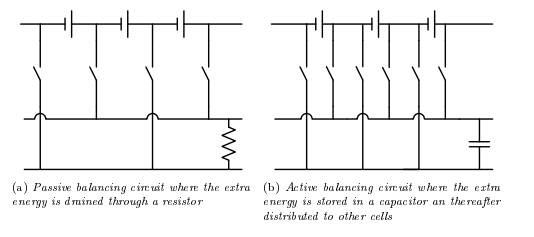
\includegraphics[scale=0.8]{Figures/balancecircuit}
\caption{Balancing circuits, source: \cite{master_thesis}}
\label{fig_circuits}
\end{figure}

Furthermore, in Daowd et al, \cite{balancing}, they describe multiple methods, both passive and active, for balancing a battery. 
One such method, Daowd et al describes, could be the Double-Tiered Switched Capacitor, figure~\ref{fig_capacitor}, which uses 2n switches and n capacitors for n cells. Compared to the active circuit in figure~\ref{fig_circuits}, the double tiered switched capacitor can reduce the balancing time by a quarter. Both, however, works in both charging and discharging operation.

\begin{figure}[H]
\centering
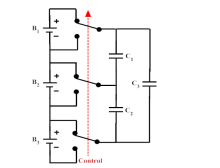
\includegraphics[scale=0.8]{Figures/capacitor}
\caption{Balancing circuit for switched capacitor, source: \cite{balancing}}
\label{fig_capacitor}
\end{figure}


\section{SOC estimation}


State of charge (SOC) is often handled by Coulomb count, but it can also be calculated directly from the OCV when current has not been drain from the battery for some time. Another estimation could be to measure the terminal voltage if the battery is drained with a constant current. In the file “log-2016-01-14.txt” column 12 are measurements of the voltage measured from a battery discharged at a constant current. The log file consist of battery voltage at 100 to 0 \% SOC. 

\begin{enumerate}
\item Briefly explain what is the criterias for a battery's SOC is at 0 \%.

For a battery to be at a state of SOC at 0\% it is enough one of the cells to be at 0 \%, since the total SOC is determined by the cell with the lowest SOC \cite{master_thesis}

\item Make an xy-plot showing the discharge curve of the battery voltage according to the GNSS time (column 5)


\begin{figure}[H]
\centering
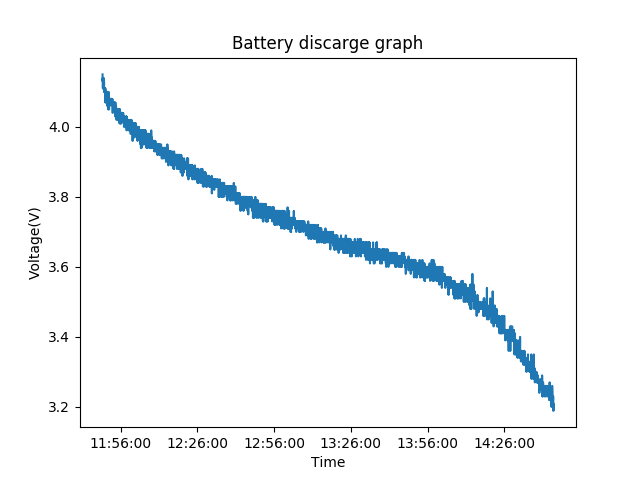
\includegraphics[scale=0.7]{Figures/batterydischarge}
\caption{Plot showing the discharge curve of the battery voltage according to time.}
\label{fig_battery}
\end{figure}

\item Create a function taking the voltage as input and the SOC as output.\\
HINT: Plot voltage on x-axis and SOC on y-axis.

The function that would describe the following figure~\ref{fig_SOC} would be of the form:
$$ SOC = {e}^{-x^2}-x $$. 
This would only be an approximation though and not nearly accurate enough.

\begin{figure}[H]
\centering
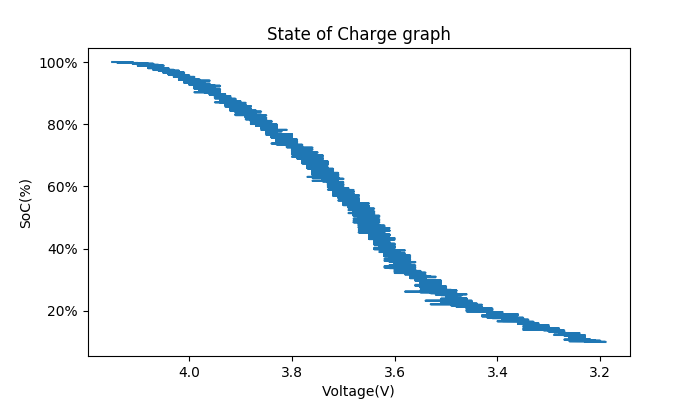
\includegraphics[scale=0.7]{Figures/StateOfCharge}
\caption{SOC vs. voltage}
\label{fig_SOC}
\end{figure}

\end{enumerate}

\pagebreak

\bibliographystyle{plain}
\bibliography{bibfile}
%----------------------------------------------------------------------------------------
%\end{multicols}
\end{document}
